\section{Background}
\frame {
    \frametitle{Vector Boson Fusion (VBF)}

    \begin{columns}
        \begin{column}{0.5\textwidth}
            \begin{tikzpicture} \begin{feynman}
                \vertex (a);
                \vertex [right=of a] (b) {H};
                \vertex [above left=of a] (vb1);
                \vertex [below left=of a] (vb2);
                \vertex [left=of vb1] (q1i) {q};
                \vertex [left=of vb2] (q2i) {q};
                \vertex [above =of b] (q1f) {q};
                \vertex [below =of b] (q2f) {q};

                \diagram* {
                    (q1i) -- (vb1) -- (q1f),
                    (q2i) -- (vb2) -- (q2f), 
                    (vb1) -- [boson] (a) -- [boson] (vb2),
                    (a) -- [scalar] (b),
                };
            \end{feynman} \end{tikzpicture}
        \end{column}
        \begin{column}{0.5\textwidth}
            VBF is the second highest Higgs production mechanism, but with a much cleaner signal than ggF
            %TODO: WHYYY is ggF not clean (maybe you don't need any pictures, but you should at least know for yourself... maybe you do need pictures though)

            \begin{figure}
                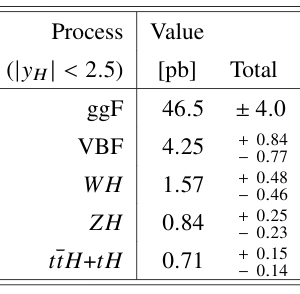
\includegraphics[width=\linewidth,height=0.5\textheight,keepaspectratio]{higgs_production_modes.png}
                \caption{source - arXiv:1909.02845 [hep-ex] }
            \end{figure}
        \end{column}
    \end{columns}
}


\frame {
    \frametitle{How is VBF Currently Handled?}

    VBF->H->diphoton (source: DOI: 10.1103/PhysRevD.98.052005)
    \begin{quote}
        Events are required to contain at least two hadronic jets,
        and the selections applied are based on the two leading jets $(j_1, j_2)$ in the event.
    \end{quote}


    % Show the different event selection rules for VBF->H->[bb,gamgam,invis]
}


\frame {
    \frametitle{The Complication of Many Jets}
    \begin{columns}
        \begin{column}{0.5\textwidth}
            \underline{\large Initial State Radiation (ISR)} \\ \vspace{5mm}
            \resizebox{0.95\textwidth}{!}{\begin{tikzpicture} \begin{feynman}
                \vertex (a);
                \vertex [right=of a] (b) {H};
                \vertex [above left=of a] (vb1);
                \vertex [below left=of a] (vb2);
                \vertex [left=of vb1] (q1i) {q};
                \vertex [below left=of vb2] (q2k);
                \vertex [left=of q2k] (q2i) {q};
                \vertex [above =of b] (q1f) {q};
                \vertex [below =of b] (q2f) {q};
                \vertex [below =of q2f] (g) {g (ISR)};

                \diagram* {
                    (q1i) -- (vb1) -- (q1f),
                    (q2i) -- (q2k) -- (vb2) -- (q2f),
                    (q2k) --[gluon] (g),
                    (vb1) -- [boson] (a) -- [boson] (vb2),
                    (a) -- [scalar] (b),
                };
            \end{feynman} \end{tikzpicture}}
        \end{column}
        \begin{column}{0.4\textwidth}
            \underline{\large Final State Radiation (FSR)} \\ \vspace{5mm}
            \resizebox{0.95\textwidth}{!}{\begin{tikzpicture} \begin{feynman}
                \vertex (a);
                \vertex [right=of a] (b) {H};
                \vertex [above left=of a] (vb1);
                \vertex [below left=of a] (vb2);
                \vertex [left=of vb1] (q1i) {q};
                \vertex [left=of vb2] (q2i) {q};
                \vertex [below right=of vb2] (q2k);
                \vertex [above =of b] (q1f) {q};
                \vertex [below =of b] (q2f) {q};
                \vertex [below =of q2f] (g) {g (FSR)};

                \diagram* {
                    (q1i) -- (vb1) -- (q1f),
                    (q2i) -- (vb2) -- (q2k) -- (q2f), 
                    (q2k) --[gluon] (g),
                    (vb1) -- [boson] (a) -- [boson] (vb2),
                    (a) -- [scalar] (b),
                };
            \end{feynman} \end{tikzpicture}}
        \end{column}
    \end{columns}
}

            % Show your table of how common this is (~20%)



